\section{Lab Tasks: Attacks}
\subsection{Task 1: Observing HTTP Request}
%
\begin{figure}
    \centering
    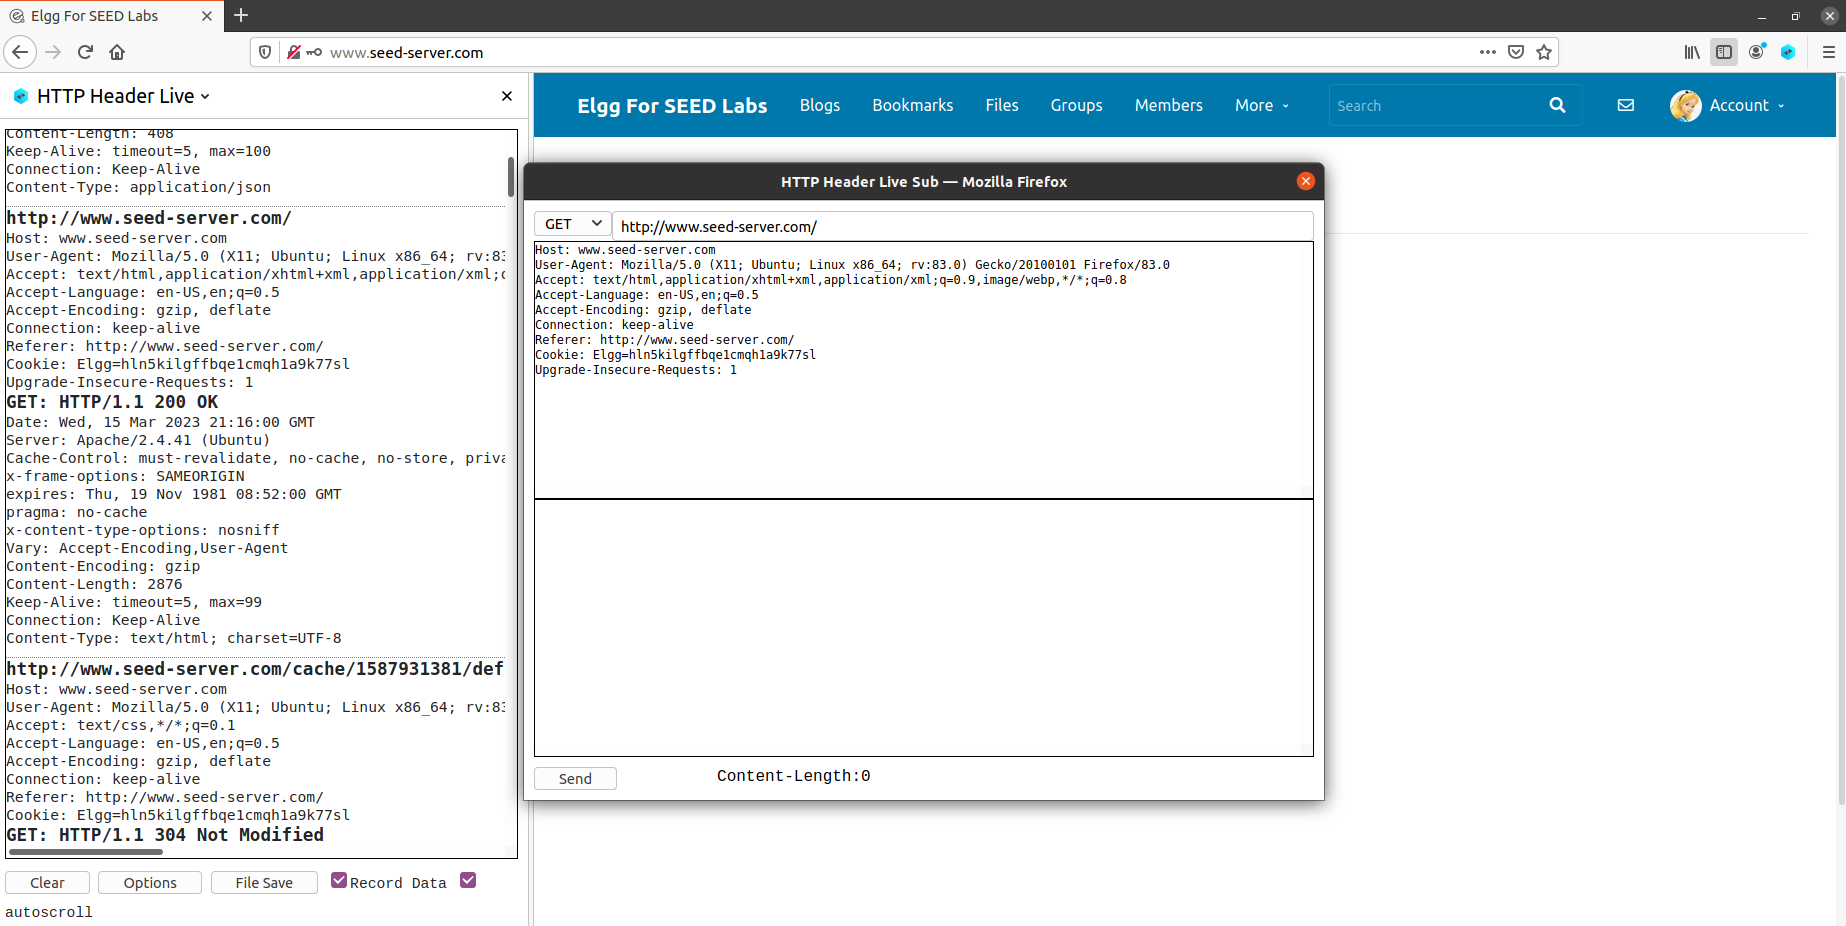
\includegraphics[width=\textwidth,height=\textheight,keepaspectratio]
    {figures/HTTP_GET.png}
    \caption{HTTP GET request in Elgg.}\label{fig:http_get}
\end{figure}

\begin{figure}
    \centering
    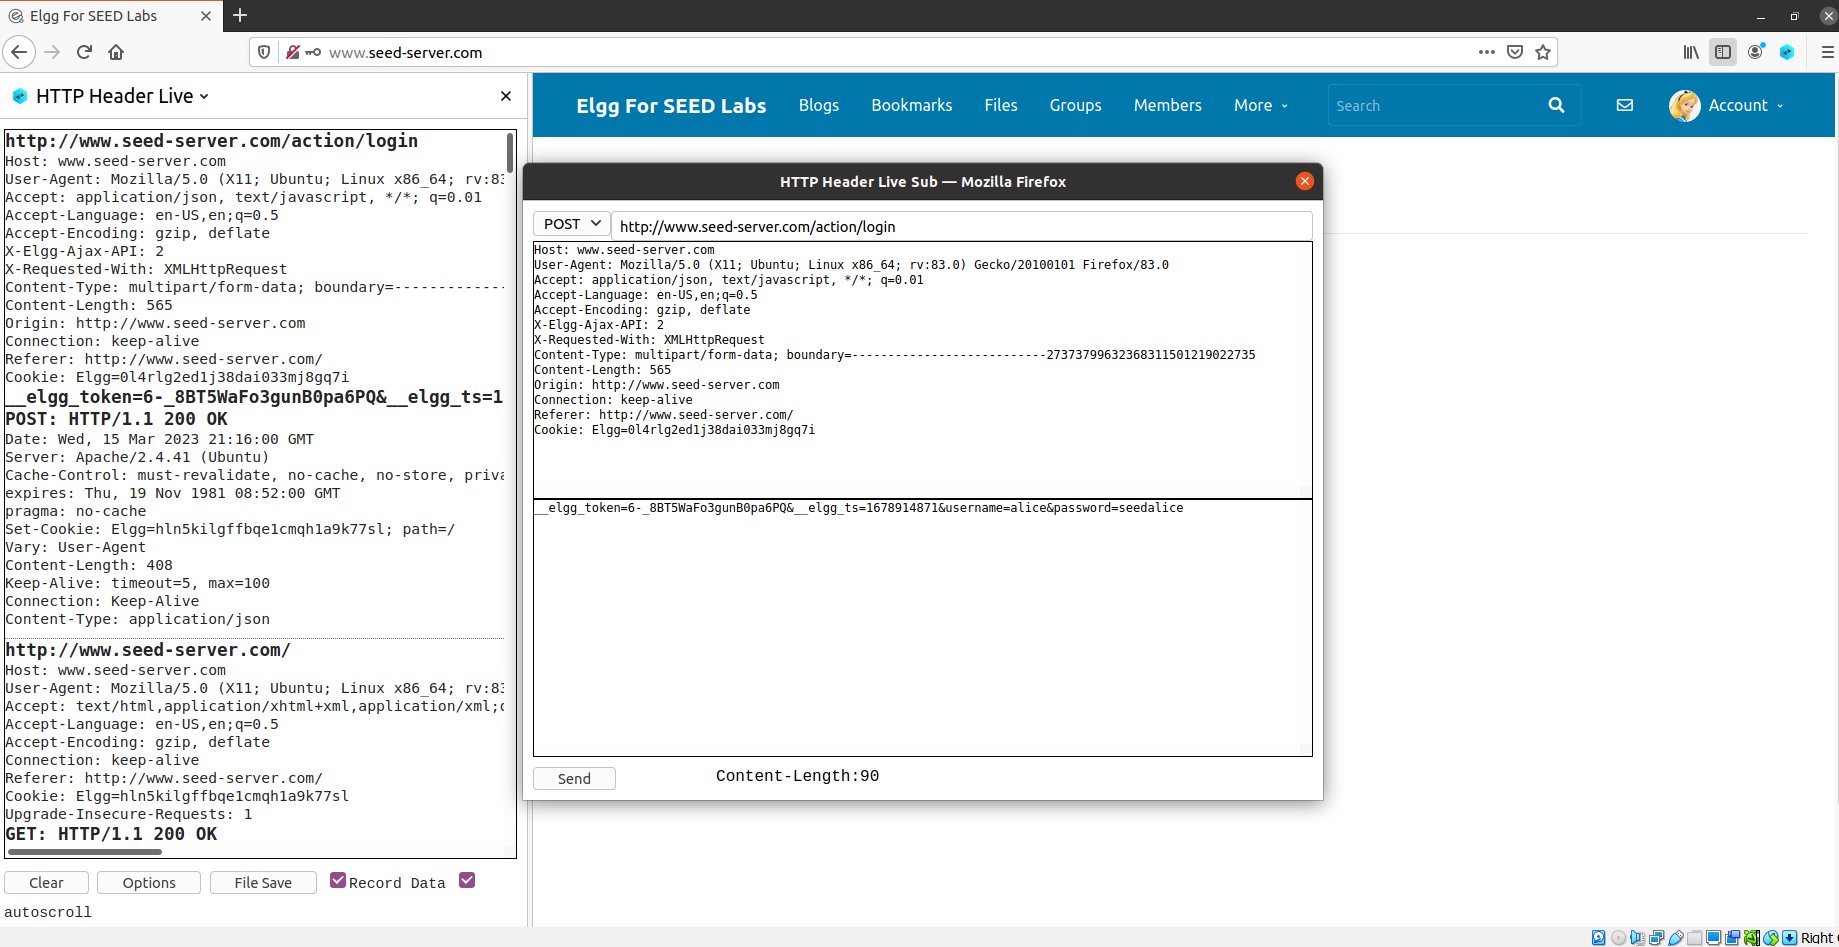
\includegraphics[width=\textwidth,height=\textheight,keepaspectratio]
    {figures/HTTP_POST.png}
    \caption{HTTP POST request in Elgg.}\label{fig:http_post}
\end{figure}

In the HTTP POST request, in this case we was trying to log in with a valid
authentication (username: \emph{alice}, password: \emph{seedalice}), it requires
a pair of parameters:{\fontfamily{qcr}\selectfont username},
{\fontfamily{qcr}\selectfont password}, {\fontfamily{qcr}\selectfont \_\_elgg\_token}, and
{\fontfamily{qcr}\selectfont \_\_elgg\_ts} (see \autoref{fig:http_post}). However, only
{\fontfamily{qcr}\selectfont username} and {\fontfamily{qcr}\selectfont password}
are inserted by a user.
On the other hand, a HTTP GET request does not require any parameters
(see \autoref{fig:http_get}).